%%
%% This is file `sample-sigconf.tex',
%% generated with the docstrip utility.
%%
%% The original source files were:
%%
%% samples.dtx  (with options: `sigconf')
%% 
%% IMPORTANT NOTICE:
%% 
%% For the copyright see the source file.
%% 
%% Any modified versions of this file must be renamed
%% with new filenames distinct from sample-sigconf.tex.
%% 
%% For distribution of the original source see the terms
%% for copying and modification in the file samples.dtx.
%% 
%% This generated file may be distributed as long as the
%% original source files, as listed above, are part of the
%% same distribution. (The sources need not necessarily be
%% in the same archive or directory.)
%%
%% The first command in your LaTeX source must be the \documentclass command.
\documentclass[sigconf, nonacm, natbib, screen, balance=False]{acmart}

% Documentation for packages
% - ACM Article Template
%    https://www.acm.org/publications/proceedings-template
% - Pseudocode typesetting CLRS-style:
%    https://www.cs.dartmouth.edu/~thc/clrscode/clrscode3e.pdf
% - Python code typesetting
%    http://ctan.uib.no/macros/latex/contrib/listings/listings.pdf
% - AMS Math
%    http://ctan.uib.no/macros/latex/required/amsmath/amsldoc.pdf
% - Graphics
%    http://ctan.uib.no/macros/latex/required/graphics/grfguide.pdf

\usepackage{url}
\begingroup
\makeatletter
\g@addto@macro{\UrlSpecials}{%
  \endlinechar=13 \catcode\endlinechar=12
  \do\%{\Url@percent}\do\^^M{\break}}
 \catcode13=12 %
 \gdef\Url@percent{\@ifnextchar^^M{\@gobble}{\mathbin{\mathchar`\%}}}%
\endgroup %


\usepackage{makecell}
\renewcommand\theadalign{bc}
\renewcommand\theadfont{\bfseries}
\renewcommand\theadgape{\Gape[0pt]}
\renewcommand\cellgape{\Gape[0pt]}

%\usepackage[colorinlistoftodos]{todonotes}
\usepackage[disable]{todonotes}
\setlength {\marginparwidth }{2cm}

\usepackage{amsmath} 

\usepackage{clrscode3e}  
\usepackage{listings}
\lstset{language=Python, basicstyle=\ttfamily}

% based on https://tex.stackexchange.com/questions/279240/float-for-lstlisting
\usepackage{float}
\floatstyle{ruled}
\newfloat{listing}{tbph}{lop}
\floatname{listing}{Listing}
\def\lstfloatautorefname{Listing} % needed for hyperref/auroref

\citestyle{acmauthoryear}
\settopmatter{printfolios=true}  % show page numbers

%% end of the preamble, start of the body of the document source.
\begin{document}

%%
%% The "title" command has an optional parameter,
%% allowing the author to define a "short title" to be used in page headers.
\title{Spring Wheat Yield prediction based on UAV Imagery}
\subtitle{Data Science Report, NMBU, Spring 2021}

\author{Muhammad Fahad Ijaz}
\email{muhammad.fahad.ijaz@nmbu.no}

%% The abstract is a short summary of the work to be presented in the
%% article.
\begin{abstract}
  This report is a part of the vPheno (virtual phenotyping) project at NMBU, started 2017. The aim of the project is to employ the image analysis and machine learning techniques to reduce the time to develop more robust cultivars, which is anywhere around 7 to 15 years by current practices. Using the data that has been collected as part of this project, I tried to develop machine learning models to predict the spring wheat grain yield, using Unmanned Aerial Vehicles (UAVs) images. The extracted features from the images were employed as input to the machine learning algorithms for yield prediction. The data from different dates was integrated using Simpson's integration. The best model parameters were estimated using a brute force search. Random Forest, Gradient Boosting and CatBoost regression models showed a good capability for grain yield prediction. Suggestion are included to improve the data collection methods and, consequently, the results for future studies.
\end{abstract}

%%
%% This command processes the author and affiliation and title
%% information and builds the first part of the formatted document.
\maketitle

\section{Introduction}\label{sec:intro}

Wheat is the most important food source all around the world \citep{Igrejas2020}. The global demand for wheat is projected to more than double by the year 2050 \citep{tilman}. This stresses the need for the increase in food crops' yield. Compared to many other countries, cultivable land is limited in Norway and it costs a lot to cultivate barren land \citep{Soilcons7:online}, the better approach would be to focus on increasing the yield from the existing cultivable land. Moreover, cultivating more land would naturally cost more. So, the reason and motivation behind plant phenotyping is to increase the yield from the same fields. 

In current state of knowledge it takes something from the realm of 7-15 years to develop a new variety from scratch. The current breeding techniques are mass selection, pure-line breeding, pedigree breeding, single seed descend (SSD), double haploids (DH) to name but a few. These techniques can be used to improve certain characteristics of the plants. Some focus on the traits like nutrition contents, while other may be oriented towards improving the yield, crop maturity time, to name a few. This is a very time-consuming process and involves a substantial cost as well.

Remote sensing systems can be deployed to get information in real time and the data collected can be used for yield prediction. One such technique is to deploy Unmanned Aerial Vehicles (UAVs) to gather data from the field. That data is used to predict different characteristics of the plants. Those traits include grain yield as well. Remote sensing does not reduce the time. It is in the experimental phase with advances happening often. Remote sensing mostly aims to improve selection accuracy and the resource pool available. Selection accuracy is improved with more precise phenotyping. It can also increase resource pool available. With bigger resource pool and higher accuracy, annual genetic gains are increased and therefore, in theory, the number of cycles to get a new variety will be fewer. In general, adding UAV multispectral phenotypes to genomic prediction models usually enhances their prediction ability. My goal is to develop a model which can predict the crop yield with greater accuracy.

Remote sensing enables a non-intrusive, high-throughput monitoring of plant physiological characteristics\citep{Tattaris2016}. Remotely sensed spectral measurements are a result of the interaction between incoming radiation and target objects. It creates a characteristic signature of reflected light. Spectral indices are a function of the light absorption properties of the plant and are calculated from these signatures \citep{Tattaris2016}.

This report contributes to the research project vPheno (virtual phenomics) at the Faculty of Bioscience at NMBU. The project, started in 2017, aims to help plant breeders to reduce the time required to select better, high yield varieties of crops and speedup the process using image analysis techniques. Earlier results related to this work have been reported by \citet{burud_bleken}, \citet{grindbakken}, \citet{lied} and \cite{shafiee2021}. This report explores a different way of data integration, using Simpson's integration to aggregate the data collected 
at different dates.

The objective of this report is to generate a machine learning model that can predict wheat grain yield, based on the image data collected from the field at different times during the season.

The first section deals with the theory of the process and spectral indices. It follows the process of data collection and pre-processing, feature extraction from images and the explanation of machine learning methods. In the results section the prediction results are outlined which are discussed in the discussion section where a comparison is made to one of the previous studies by \citet{lied}.

\section{Theory}\label{sec:theory}

\subsection{Plant Phenotyping}\label{sec:plant_pheno}

Plant phenotyping is the study of how plants traits, termed as phenome, develop from their interaction with the environment and how their genome can be related to those traits \citep{minervini}. These traits include, among others, the plant yield, maturity time, plant height, etc. The importance of phenotyping has increased significantly with the increased demand for improving the yield.
Plant phenotyping investigates how the physical features are affected by the genome of the plant. Efficient and sustainable agriculture practices stress the need and importance of such methods \citep{Minervini13}.

Image-based phenotyping methods are fast and nondestructive. They can predict the results and save time to make decision about the choice of the variety of wheat to be chosen for the next phase.

\subsection{Spectral Indices}\label{sec:indices}

Spectral indices are derived values from one or more reflection bands. They are used to indicate the presence of the required features in an image and are derived by combining the spectral reflectance from multiple wavelengths of light reflected from a surface \citep{indices:online}. There are several different spectral indices. The ones related to plants are called vegetation indices \citep{huete}. Vegetation indices are designed to highlight specific properties of vegetation \citep{veg_indices:online}.For this study, we are focusing on the ones that can be derived from the spectral bands data we have gathered for the project. These indices have shown good results in predicting the grain yield \citep{Zhang2014}. The five bands, collected by the by the Micasense RedEdge-M multi-spectral camera, are listed in the Table \ref{tab:bands}.


\begin{table}[h!]
  % Table captions always come *above* .
  \caption{Table with details of bands data collected by the Micasense RedEdge-M \citep{RedEdgeM:online, lied}}
  \label{tab:bands}
  \begin{tabular}{lll}
    \hline
    Band Name & Center wavelength (nm) & Bandwidth (nm) \\\hline
    \verb!Blue! & \verb!475! & \verb!20! \\
    \verb!Green! & \verb!560! & \verb!20! \\
    \verb!Red! & \verb!668! & \verb!10! \\
    \verb!RedEdge! & \verb!717! & \verb!10! \\
    \verb!NIR! & \verb!840! & \verb!40! \\

  \end{tabular}
\end{table}






The relevant vegetation indices and the formula to calculate them are as follows.


\subsubsection{Normalized difference vegetation index - NDVI}\label{sec:ndvi}

NDVI is used for analyzing vegetation. This was calculated by measuring the difference in reflection between near–infrared (NIR) and red light (RED).  Chlorophyll is an indication of healthy vegetation. It absorbs more red light while reflects NIR and green light. NDVI is calculated using the equation \ref{eq:ndvi} \citep{rouse1974monitoring}.

\begin{equation}
  %\caption{NDVI Equation}
  \label{eq:ndvi}
NDVI=\ \frac{NIR-RED}{NIR+RED}
\end{equation}

NDVI Values range from negative one (-1) to positive one (+1). Negative values indicate water bodies and are not related to vegetation. Values approaching zero indicate no green vegetation whereas the values close to one indicate the presence of green vegetation \citep{NDVI72:online}. NDVI is an indicator of plant health.  A value between 0 and 0.33 a stressed plant, 0.33 to 0.66 is moderately healthy, and 0.66 to 1 is very healthy \citep{NDVIPlan50:online}. These numbers vary depending on the plant type and other conditions. But they can be used as a rule of thumb.

NDVI suffers from saturation problem in well vegetated areas. This is mainly because of the red band whose energy is strongly absorbed by pigments. If there is a certain amount of pigment in the leaf, the reflectance in the red band will will almost remain unchanged even if more pigment is present\citep{wang2003}.


\subsubsection{ MERIS terrestrial chlorophyll index - MTCI}\label{sec:mtci}

This index is a measure of the chlorophyll content. Spectral data indicates that important information about the leaf area index can be found in the RedEdge band. Sharp changes in the reflectance are observed between wavelengths 690 and 750 nm. So a positive change in this region is indicative of chlorophyll content in the leaf\citep{DELEGIDO201342}. MTCI integrates the red-edge band (REG) into the equation for that reason, in addition to Red and NIR, which are included in NDVI as well. MTCI is calculated by the equation \ref{eq:mtci} \citep{dash2004meris}:

\begin{equation}
  %\caption{MTCI Equation}
  \label{eq:mtci}
MTCI=\ \ \frac{NIR-RedEdge}{RedEdge-Red}
\end{equation}
  %\caption{MTCI Equation}

In comparison with NDVI, MTCI is better at yield prediction \citep{Zhang2014}. 


\subsubsection{Enhanced vegetation index - EVI}\label{sec:evi}

EVI is calculated like NDVI. However, it corrects for some distortions in the reflected light caused by particles in the air and the ground cover below the vegetation. The EVI value does not become saturated as quickly as the NDVI when viewing areas with a high amount of chlorophyll \citep{Lein2012}. EVI is calculated using the equation \ref{eq:evi} \citep{HUETE1994224, Lein2012, rs2012}.

\begin{equation}
  %\caption{EVI Equation}
  \label{eq:evi}
EVI=\ 2.5\ \times\frac{NIR-RED}{NIR+(6\times R E D)-(7.5\times B L U E)+1}
\end{equation}


\section{Method}\label{sec:method}

The data is collected from one field where different varieties of spring wheat has been planted in several sub-plots. Data collection is done by using a UAV equipped with an RGB Camera, in addition to a Micasense RedEdge-M multi-spectral camera, a GPS Module and an ambient light sensor. The UAV is flown over the field on a predefined grid pattern path and it captures the image data of the field. The image data is then stitched to get an overall image of the field. The data collected by the system consists of blue, green, red, red edge and near-infrared bands. The median band values for each band are taken for each plot and are used to calculate the vegetation indices, i.e. Normalized Difference Vegetation Index (NDVI), MERIS Terrestrial Chlorophyll Index (MTCI), and Enhanced Vegetation Index (EVI).

\subsection{Test Site}\label{sec:site}

The test site is located at Vollebekk Research Farm, close to NMBU in Ås, in south-eastern Norway. The coordinates of the site are 59°39'23.6"N 10°45'13.8"E. One spring wheat field with 96 sub-plots is included in this study. The cultivars were sown on 20th April, 2020. Twenty-four different candidate cultivars are cultivated in the sub-plots with each cultivar planted in four sub-plots. The placement of the cultivars is random with randomization being done in an alpha-lattice design \citep{Kumar2020}.


\begin{figure}[h]
  \centering
   \hspace*{-0.25in}
   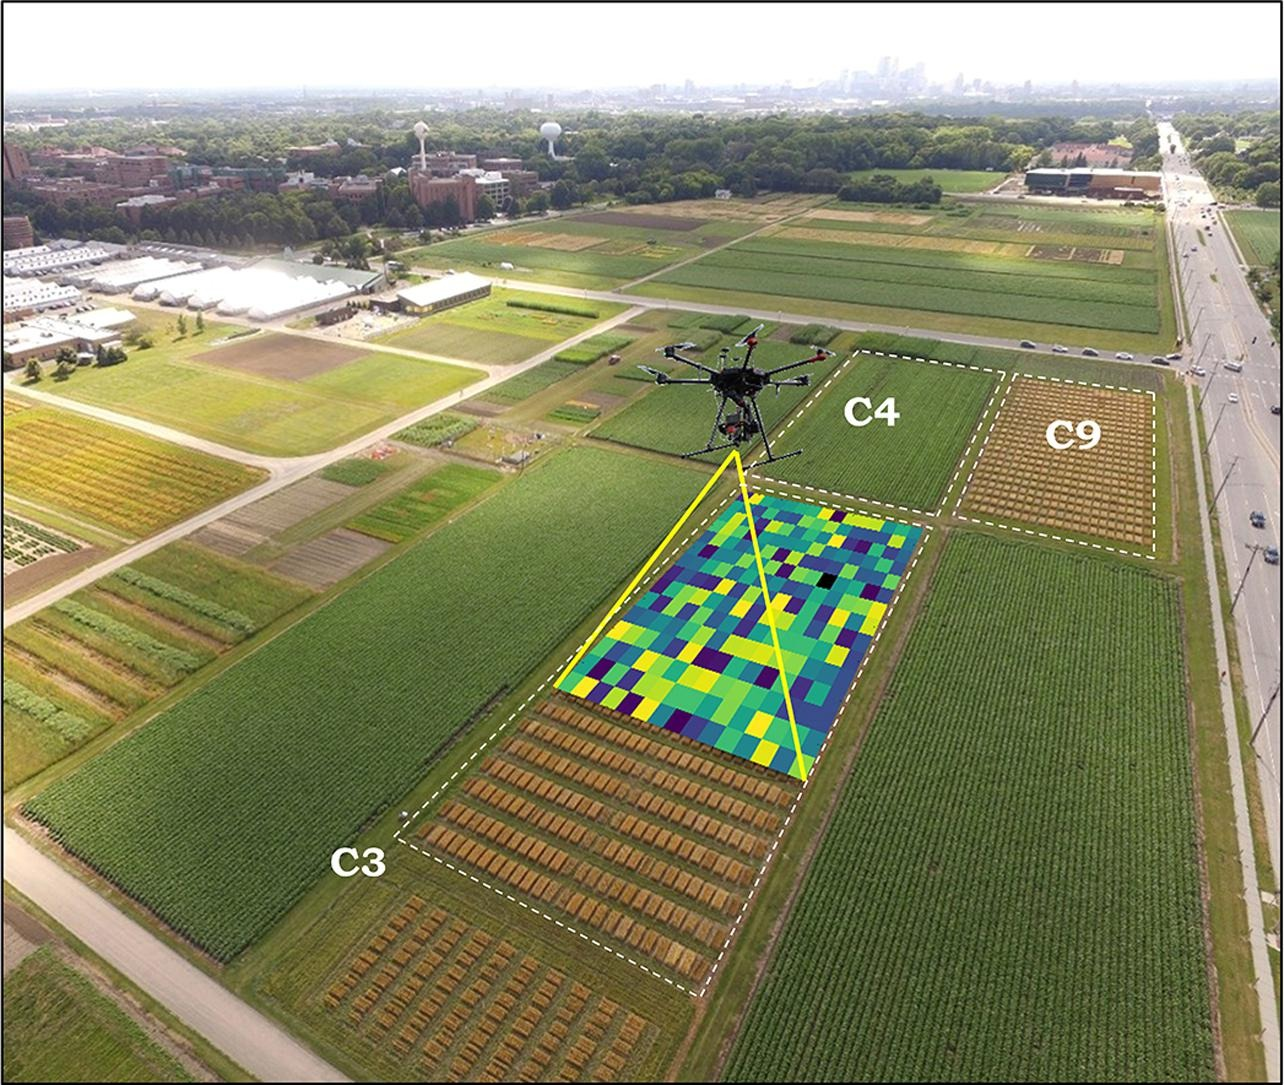
\includegraphics[width=0.4\textwidth, angle=0,]{moghimi.jpg}
  % figure captions below figure
  \caption{A illustration of the data collection process\citep{moghimi}. This illustration is to explain the data collection process and is not of the field and UAV used for this study.}
  %% Explain the size of the data used

  \label{fig:example}
\end{figure}


Each subplot is separated from the neighboring subplots by a border row. This is done to reduce the border effect \citep{May1986EFFECTOD, WANG20171}. As a standard agronomic practice, herbicides and fungicides are used on the crops to ensure better yield. In addition to the image data, manual measurements are also done to determine the number of days to maturity and number of days to heading of the plant. Heading is a growth stage of the wheat plant when the wheat head/fruit has fully emerged\citep{White2008}. Maturity comes later and is defined as the stage where the complete plant material has turned golden and is ready for harvest\citep{Hanft1982}. Plant height is also measured once before harvest, when the plants are at their maximum growth height. Grain yield is measured in $g/m^2$.

\subsection{Image Data Collection}\label{sec:data_collection}

The image data is collected by a UAV which had been mounted with necessary equipment to gather the images and multi-spectral data. The UAV used is DJI Matrice 100 \citep{Matrice171:online}. It comes with a GPS Module. Zenmuse X3 camera module from DJI is installed on the UAV which is used to gather the RGB image data. The RGB Camera has a 1/2.3” CMOS sensor with 12.4 effective megapixels \citep{ZenmuseX77:online}. In addition to that, a RedEdge Downwelling Light Sensor (DLS) \citep{light_sensors:online} from Micasense and a RedEdge-M multi-spectral by Micasense \citep{RedEdgeM:online} are used as well \citep{lied}. The image resolution of the RGB camera is $3000 \times 4000$ pixels.

The lighting conditions vary from season to season, depending on weather. This affects the consistency of the collected data. This effect needs to be compensated to acquire reliable data in the long run. The ambient light sensors are used to compensate for this variation \citep{Bestpractices_mica:online}.

\subsection{Image Processing}\label{sec:image_proc}

Pix4D and QGIS are the software's used to process the image data and convert it into tabular form to be used for machine learning. After the images are collected using the equipment described, the next step is to stitch them together to form one big reflectance map of the field. This is done in Pix4D. This is detailed in \citet{lied} and \citet{grindbakken}.

The QGIS application is used to extract the required data from the reflectance map generated from the data collected from the cameras on the UAV. Geographical Information Systems are commonly referred to as GIS. QGIS is an open-source GIS application. Geo-processing, sampling and vector analysis are some of the applications of QGIS. For processing the reflectance map, a custom grid is generated, using QGIS, matching the setup of subplots in the field \citep{lied}. It extracts the required values of the bands for each subplot from the grid. It was used to plot and index the median value of pixels in each sub-plot. The data is exported to a csv file.

\subsection{Detail of available data}\label{sec:detail_data}

Table \ref{tab:samples} is representing the dataset for the current study. The data collected in dates between heading and maturity is of most importance since it is more relevant and practical to use that data for yield predictions \cite{shafiee2021}.

\begin{table}[h!]
  % Table captions always come *above* .
  \caption{Remote sensing data Robot Field}
  \label{tab:samples}
  \begin{tabular}{|c|c|c|}
    \hline

    \textbf{Date} & \textbf{No. of Sub-plots} & \textbf{Comments} \\
    \hline

    18/06/2020 & 96 & Complete\\    \hline
    23/06/2020 & 96 & Complete \\ \hline
    24/06/2020 & 96 & Complete \\    \hline
    25/06/2020 & 96 & Complete \\    \hline
    29/06/2020 & 96 & Complete \\    \hline
    01/07/2020 & 96 & Complete \\    \hline
    07/07/2020 & 96 & Complete \\    \hline
    13/07/2020 & 96 & Complete \\    \hline
    16/07/2020 & 96 & NIR data missing \\    \hline
    20/07/2020 & 96 & Complete \\    \hline
    22/07/2020 & 96 & Complete \\    \hline
    27/07/2020 & 96 & Complete \\    \hline
    30/07/2020 & 96 & Complete \\    \hline
    04/08/2020 & 96 & \makecell{After\\maturity}\\    \hline
    07/08/2020 & 96 & \makecell{After\\maturity}\\    \hline
    12/08/2020 & 96 & \makecell{After\\maturity}\\    \hline
    14/08/2020 & 96 & \makecell{After\\maturity}\\

    \hline

  \end{tabular}
\end{table}

NIR data was missing in one of the dates which was dropped. Twelve remaining datasets marked 'Complete' in Table \ref{tab:samples} were used for further processing.

\subsection{Data Features}\label{sec:processing}

The features in the available datasets are listed in Table \ref{tab:input_variables}. Eight features have been used as input features while grain yield is the target variable. There are other features also available from the data. For example, maturity, plant height, protein content, etc. but these can only be determined at a later stage of growth. Since, in a real-world scenario, this data will not be available to the model while making predictions for new data, these were not included in model training. Heading is a feature that is available before harvest. It was not used since it is practically the same for all sub-plots in this field. It can be useful to include this when using the data from multiple fields. Since in this case, we have the date from only one field, this was not used for model training and evaluation.


\begin{table}[h!]
  % Table captions always come *above* .

  \caption{Details of Features from the dataset}
  \label{tab:input_variables}

  \begin{tabular}{|c|c|c|c|} \hline
	\textbf{Name} & \textbf{Explanation} & \textbf{Selection} & \textbf{Type} \\\hline
    \multicolumn{4}{|c|}{\textbf{Input Features}} \\\hline

	Blue & Blue band & Median & Band Data  \\\hline
	Green & Green Band & Median & Band Data \\\hline
	Red & Red Band & Median & Band Data \\\hline
	Red Edge & \makecell{Red-NIR\\transition zone}  & Median & Band Data \\\hline
	NIR & Near Infrared & Median & Band Data \\\hline
	NDVI & \makecell{Normalized Difference\\Vegetation Index} & Median & \makecell{Vegetation \\index} \\\hline
	MTCI & \makecell{The MERIS\\terrestrial \\chlorophyll index} & Median & \makecell{Vegetation \\index} \\\hline
	EVI & \makecell{Enhanced vegetation\\index} & Median & \makecell{Vegetation \\index} \\\hline

    \multicolumn{4}{|c|}{\textbf{Target Variable}} \\\hline
    \makecell{Grain\\Yield} & Grain Yield in $g/m^2$ & - & \makecell{Target\\Variable}\\\hline
    
    \multicolumn{4}{|c|}{\textbf{Features applicable post-harvest (except heading)}} \\\hline
    \makecell{Heading} & \makecell{Days to heading\\from sowing} & - & Days\\\hline
    \makecell{Maturity} & \makecell{Days to maturity \\from sowing} & - & Days\\\hline
    \makecell{Plant \\height} & \makecell{Plant height\\at maturity\\in cm} & - & cm\\\hline
    \makecell{Protein\\content} & \makecell{Protein content\\in \%} & - & \%\\\hline
    \makecell{Spikes} & \makecell{Number of Spikes\\ per $m^2$
} & - & Number\\\hline
    
  \end{tabular}
\end{table}


\subsection{Data pre-processing}\label{sec:preprocessing}

Each sub-plot has a single median value for each band for which the data has been collected in the images. This is generated from the pixels of each sub-plot. The reason for using the median values for all bands is because median values are not affected much by outliers' presences in the data. Median value can compensate for the presence of soil pixels in the image, whose band values would be on a different than of the pixels for the vegetation.


\subsubsection{Irregularities in the data}\label{sec:nan}

All the bands data from each date was plotted as box plots. Examining the plots, it is clear that the data from 29-Jun does not follow the trends in all the bands. There might be some problems with data collection process. The data from this date has been dropped from further investigation. Remaining eleven datasets have been used further.

\begin{figure}[!h]
   \hspace*{-0.25in}
   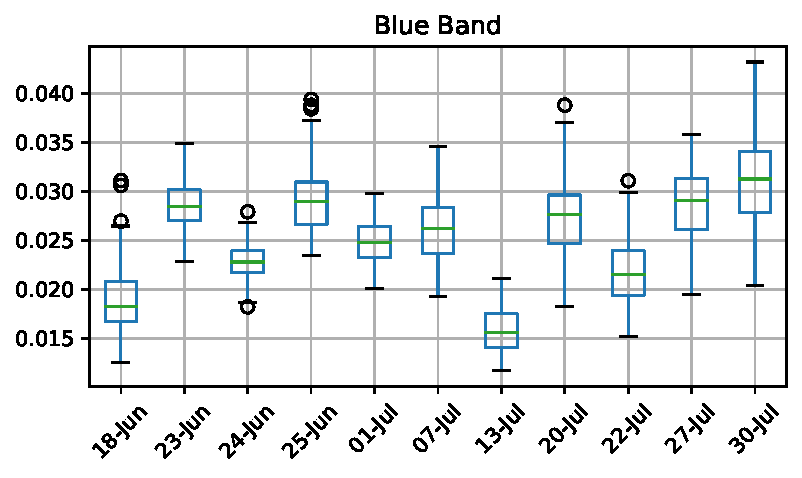
\includegraphics[width=0.5\textwidth, angle=0,]{Blue.pdf}
  \caption{Boxplots of Blue Band data from all datasets}
  \label{fig:blue}
\end{figure}

\begin{figure}[!h]
   \hspace*{-0.25in}
   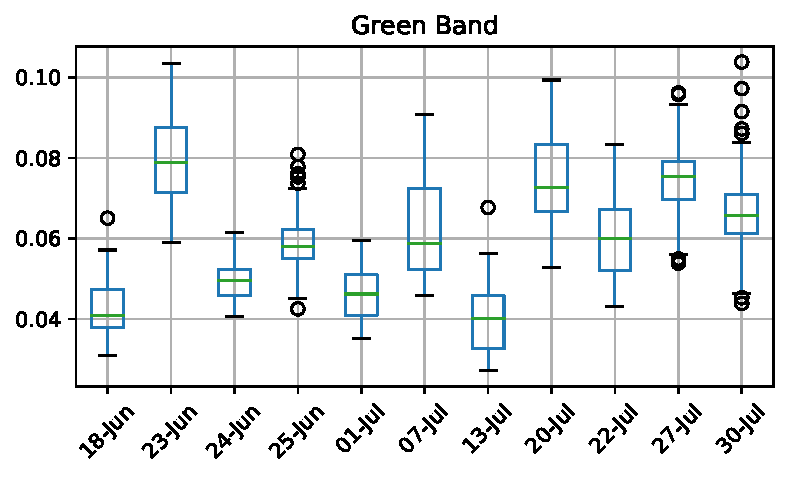
\includegraphics[width=0.5\textwidth, angle=0,]{Green.pdf}
  \caption{Boxplots of Green Band data from all datasets}
  \label{fig:green}
\end{figure}

\begin{figure}[!h]
   \hspace*{-0.25in}
   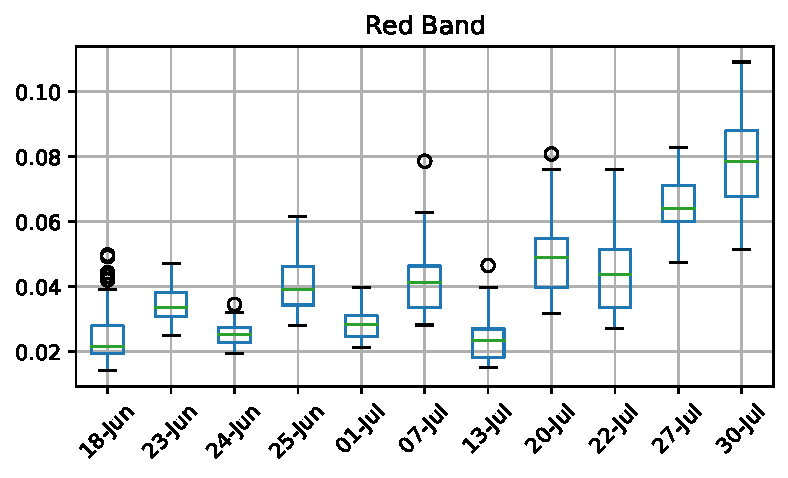
\includegraphics[width=0.5\textwidth, angle=0,]{Red.pdf}
  \caption{Boxplots of Red Band Data from all datasets}
  \label{fig:red}
\end{figure}

\begin{figure}[!h]
   \hspace*{-0.25in}
   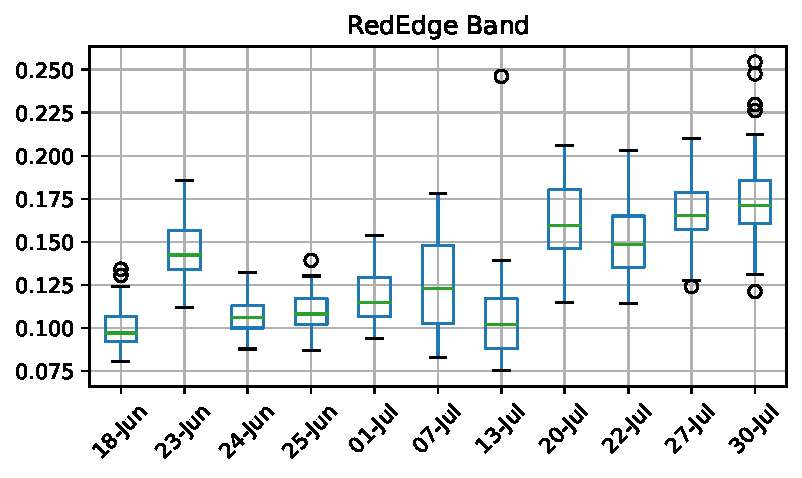
\includegraphics[width=0.5\textwidth, angle=0,]{RedEdge.pdf}
  \caption{Boxplots of RedEdge Band data from all datasets}
  \label{fig:rededge}
\end{figure}

\begin{figure}[!h]
   \hspace*{-0.25in}
   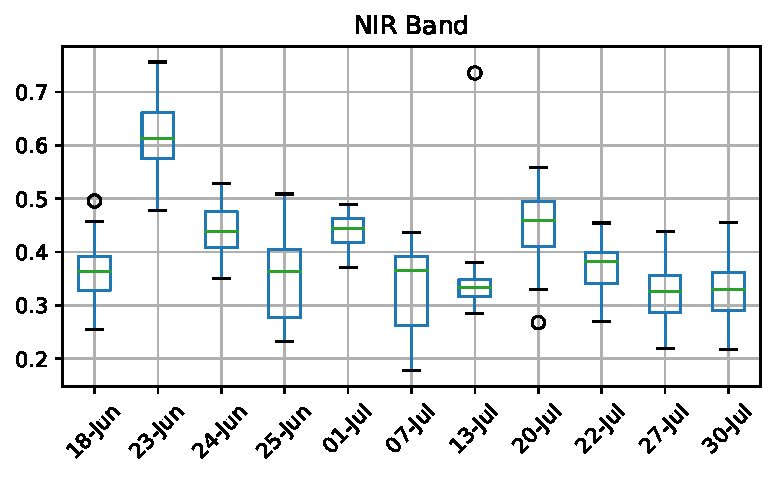
\includegraphics[width=0.5\textwidth, angle=0,]{NIR.pdf}
  \caption{Boxplots of NIR Band data from all datasets}
  \label{fig:nir}
\end{figure}

\subsubsection{Data Compilation Strategy}\label{sec:strategy}

The previous studies on similar data at NMBU \cite{burud_bleken}, \cite{grindbakken} and \cite{lied}, \cite{shafiee2021} have taken a different approach to data compilation for machine learning. They compiled the data sets by adding the data collected on different dates as new features in the dataset. This resulted in an enormous increase in the number of features in the dataset, but the number of samples remained the same. The reasoning for this strategy was that since for one plot, although the data is being collected several times in one season, but at the end of the season, one sub-plot has only one grain yield value. So, it is better to add new features to the same samples than to add them as new samples as all the feature of one sub-plot correspond to the same grain yield.

I took a different approach by integrating the data for each subplot by using Simpson's Integration\cite{Simpsons2:online}. It uses the number of days from sowing for each date and integrates all the values for one band into a single value by calculating the area under the band value and number of days curve. It integrated the 11 values for each band for one plot into one integrated value. So, for the 96 sub-plots, there are eight input features which are the integration of the same features of the data from ten different dates. 

In case of multiple fields, the data collected is not usually equally spaced in time. There are several practical reason for not being able to collect data as planned. Weather plays an important role. Data is usually not collected on a cloudy day or during bad weather or rain. The real world data ends up not equally spaced thus not comparable from one season to the other. By integrating the data, we can get a comparable approximation of the data if there are same number of days between the first and last date of data collection.

Figure \ref{fig:heatmap} shows the correlation between all the input features and with the target variable,i.e. grain yield.

\begin{figure}[!h]
   \hspace*{-0.25in}
   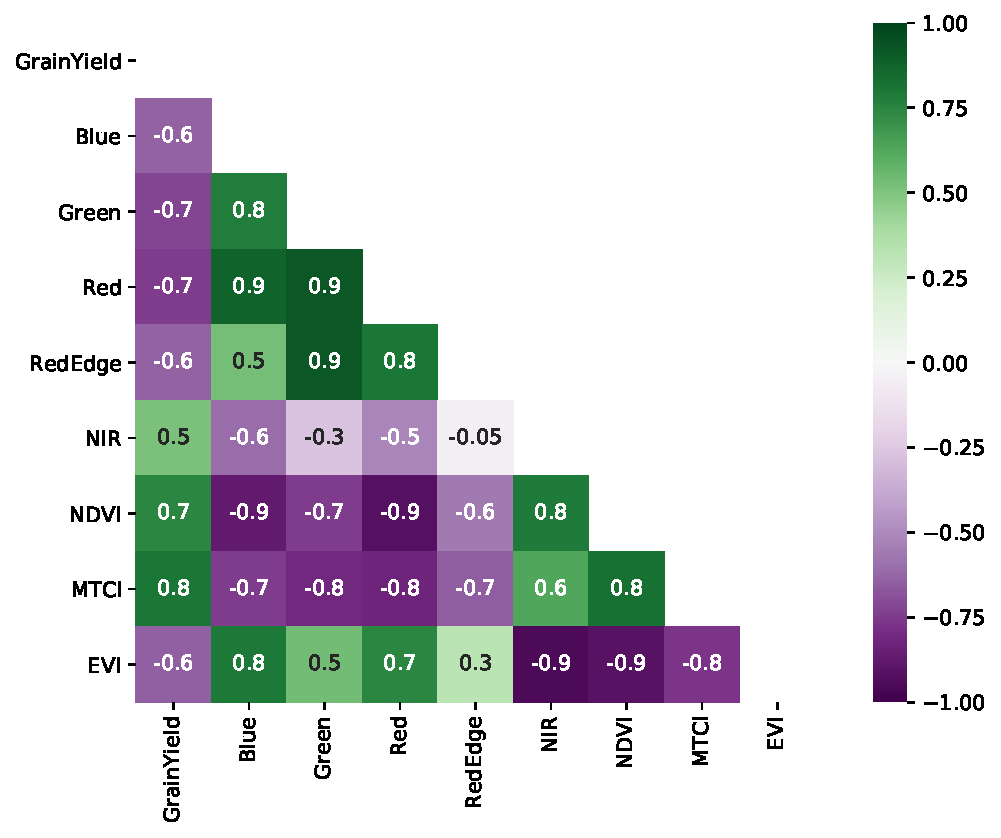
\includegraphics[width=0.55\textwidth, angle=0,]{heatmap.pdf}
  \caption{Pearson Correlation Heat map indicating the correlation between the input and target variables}
  \label{fig:heatmap}
\end{figure}


\subsection{Machine Learning}\label{sec:ml}

The machine learning analysis has been programmed in Python programming language \citep{python3}. The machine learning algorithms are from Scikit-Learn (0.23.2) \citep{scikit-learn} and CatBoost (version 0.24.3) \citep{cat2018} libraries. The analysis and predictions have been executed in a Jupyter Notebook \citep{Kluyver2016jupyter} with Python version 3.8.5.

\subsubsection{Git hashes}


\begin{table}[h!]
  % Table captions always come *above* the table.
  \caption{Versions of files used for this report; Gitlab repository
    \url{https://gitlab.com/fahadijaz/ds-report-spring-2021}}
  \label{tab:hashes}
  \begin{tabular}{ll}
    \hline
    File & Git hash \\\hline
    \verb!1. Data Cleaning.ipynb! & \verb!4d06c51a! \\
    \verb!2. ML-Simps Integration.ipynb! & \verb!b50c6a21! \\ \hline
  \end{tabular}
\end{table}


\subsubsection{Sampling and data partitioning}\label{sec:sampling}

The dataset divided into trai (70\%) and test (30\%) sets. The test\_train\_split function from Scikit-Learn is used for making the split. The data is shuffled during the split. The default values of the hyperparameters are used.

Random sampling was used as a means to validate the model results. It splits the data into random splits and those splits are used to train and test the model. This was done using random seeds in the range from 0 to 9. The average of the ten results is used as measure of the prediction accuracy of the model.

\subsubsection{Standardization}\label{sec:standardization}

Standardization has been used for the Lasso model as it resulted in an improvement in the prediction accuracy. It has been done using the StandardScaler from Scikit Learn. StandardScaler scales the features to unit variance. This improves the predictions results for most of the machine learning estimators \citep[Ch.~2]{Rashka2015}. Default values have been used for the hyper-parameters for StandardScaler.

\subsubsection{Machine Learning Models}\label{sec:ml_models}

This problem requires the machine learning models to predict a continuous target. This makes it a regression problem. So, regression estimators have been used for that purpose. From Scikit learn, Lasso, Random Forest Regressor and Gradient Boosting Regressor are used. In addition, CatBoostRegressor is also used.

% \subsubsubsection{Lasso Regression}


% \subsubsubsection{Random Forest Regressor}
Random forest is an ensemble model. It combined multiple decision trees and aggregate their results using a statistical technique called bagging, to formulate the results. This technique results in a robust model that is less prone to over fitting \cite{Varghese18:online}. Random Forest comes up with a robust, accurate model that can handle large varieties of input data with binary, categorical, continuous features.

% \subsubsubsection{Gradient Boosting and CatBoost}
Gradient Boosting Machines (GBMs) is explained by two concepts: Decision trees and boosting. Decision trees are machine learning models which use specific connections between variables to classify the data points correctly. Boosting is a technique that creates several decision trees based on the results of the previous trees. For every tree made, a greater weight is put on the changing/altering of the weights that are hard to classify. Gradient Boosting Machines uses a cost function to determine the properties of each subsequent tree \cite{gb18:online}.

CatBoost uses a Gradient Boosting algorithm for prediction of the classifier. It uses a framework for gradient boosting based on decision trees\cite{CatBoost90:online}.

\subsubsection{Model Evaluation}\label{sec:evaul}

For model evaluation, Coefficient of Determination ($R^2$), Mean Absolute Error and Root Mean Squared Error(RMSE) and were used.

The coefficient of determination is a measure of regression score where the best possible score is 1.0. The values lower than that indicate worse prediction results.

RMSE determines the regression loss. It is calculated adding the squared difference between the prediction and the target variable and dividing the sum by the number of samples. The square root of the resulting value is the RMSE.

MAE is a measure of the average magnitude of error in the predictions. It is calculated adding the absolute difference between the prediction and the target variable and dividing the sum by the number of samples.

\subsubsection{Hyperparameters Tuning}\label{sec:evaul}
The hyperparameters of the models were tuned one by one using Brute force search method. One hyperparameter was tuned based on the \textit{r2\_score} metric from sklearn. The search was carried out step by step, tuning one parameter at a time.  The best hyperparameters of each of models are given in Table \ref{tab:lasso}, Table \ref{tab:rfr}, Table \ref{tab:gbr} and Table \ref{tab:catbr}.

\begin{table}[h!]
  % Table captions always come *above* the table.
      \caption{Hyperparameters of Lasso Model}
  \label{tab:lasso}
  \begin{tabular}{ll}
    \hline
    Hyperparameter & Value \\\hline
    \verb!alpha! & \verb!4.5! \\ \hline
  \end{tabular}
\end{table}

\begin{table}[h!]
  % Table captions always come *above* the table.
      \caption{Hyperparameters of RandomForestRegressor Model}
  \label{tab:rfr}
  \begin{tabular}{ll}
    \hline
    Hyperparameter & Value \\\hline
    \verb!max_depth! & \verb!250! \\
    \verb!min_samples_split! & \verb!14! \\
    \verb!min_samples_leaf! & \verb!3! \\
    \verb!random_state! & \verb!1! \\ \hline
  \end{tabular}
\end{table}

\begin{table}[h!]
  % Table captions always come *above* the table.
      \caption{Hyperparameters of GradientBoostingRegressor Model}
  \label{tab:gbr}
  \begin{tabular}{ll}
    \hline
    Hyperparameter & Value \\\hline
    \verb!subsample! & \verb!0.8! \\
    \verb!learning_rate! & \verb!0.4! \\
    \verb!random_state! & \verb!500! \\
    \verb!random_state! & \verb!1! \\ \hline
  \end{tabular}
\end{table}

\begin{table}[h!]
  % Table captions always come *above* the table.
      \caption{Hyperparameters of CatBoostRegressor Model}
  \label{tab:catbr}
  \begin{tabular}{ll}
    \hline
    Hyperparameter & Value \\\hline
    \verb!depth! & \verb!8! \\ \hline
  \end{tabular}
\end{table}

In terms of hyperparameter tuning, most of the hyperparameter performed the best with their default values. Tuning them did not result in any improvement in their accuracy. Those of them which resulted in better predictions have been used and reported in this report.



\section{Results}\label{sec:results}

This report investigates the potential of using Simpson's integration technique for aggregating the data from several dates to accurately predict the grain yield of spring wheat. In addition, this report also evaluates the ability of the vegetation indices to make yield prediction.


\subsection{Evaluation Results}\label{sec:ev_results}

The results from the estimators are listed in \ref{tab:results}. Standardized data, as explained in section \ref{sec:standardization}, was only used for Lasso Model. Tree based models used are not affected by any monotonic transformation of the features. So, non-transformed data was used for the remaining models.

Random Forest Regressor performed the best in terms of the three matrices in the Table \ref{tab:results}. The scores of Gradient Boosting Regressor and CatBoost Regressor are close, with CatBoost Regressor trailing just behind the Gradient Boosting Regressor. Lasso performed the worst. 

\begin{table}[h!]
  % Table captions always come *above* .
  \caption{Prediction results}
  \label{tab:results}
  \begin{tabular}{|c|c|c|c|c|}
    \hline

     \textbf{Model} & \textbf{Standardization} & \textbf{$R^2$} & \textbf{MAE} & \textbf{RMSE}  \\
    \hline

    Lasso & Yes & 0.617 & 46.29 & 58.11\\ \hline
    RandomForest & No & 0.736 & 38.21 & 48.21\\ \hline
    GradientBoosting & No & 0.714 & 38.94 & 49.96\\ \hline
    CatBoost & No & 0.713 & 39.32 & 50.28\\ \hline
  \end{tabular}
\end{table}

\subsection{Feature Importance}\label{sec:feat_imp}

The feature importance from the regression models used is plotted in Fig. \ref{fig:festure_rf}, Fig. \ref{fig:festure_gb} and Fig. \ref{fig:festure_cb}. Lasso model from Scikit learn does not have a method to return the feature importance of the input features.

\begin{figure}[!h]
   \hspace*{-0.25in}
   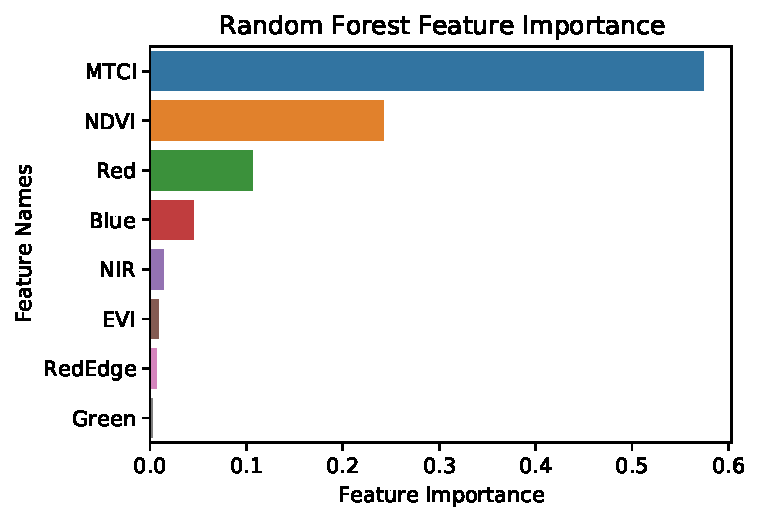
\includegraphics[width=0.5\textwidth, angle=0,]{feature_importance_RF.pdf}
  \caption{Feature Importance of Simpson's integrated vegetation indices calculated by the Random Forest model}
  \label{fig:festure_rf}
\end{figure}

\begin{figure}[!h]
   \hspace*{-0.25in}
   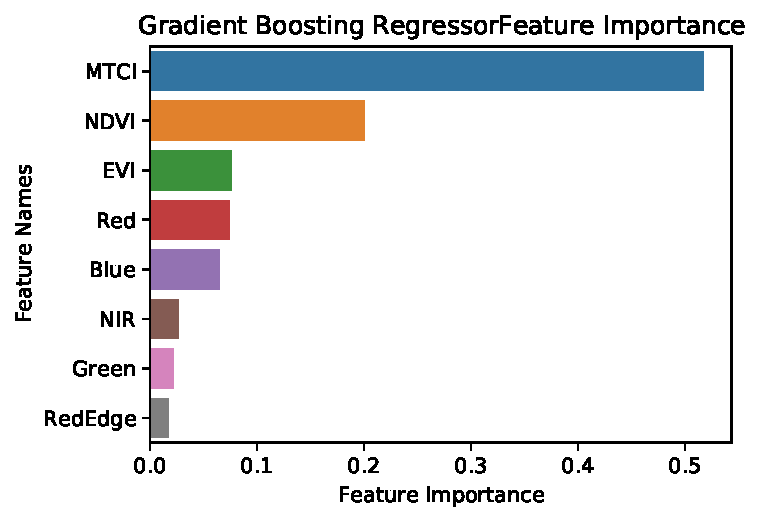
\includegraphics[width=0.5\textwidth, angle=0,]{feature_importance_GB.pdf}
  \caption{Feature Importance of Simpson's integrated vegetation indices calculated by the Random Forest model}
  \label{fig:festure_gb}
\end{figure}

\begin{figure}[!h]
   \hspace*{-0.25in}
   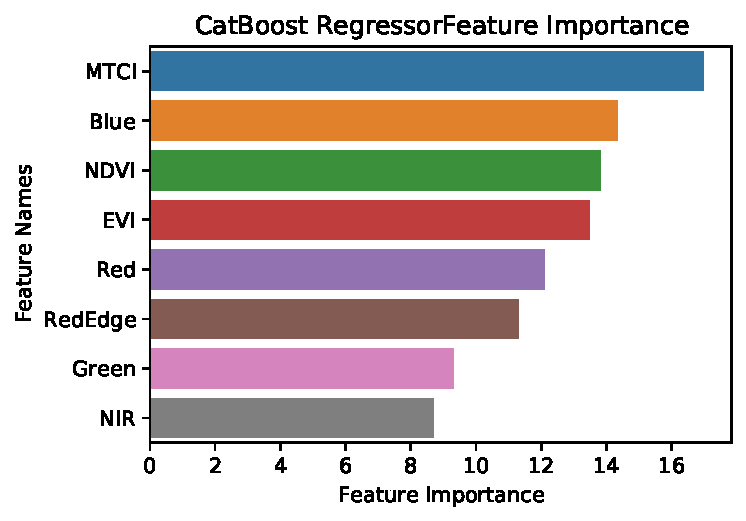
\includegraphics[width=0.5\textwidth, angle=0,]{feature_importance_CB.pdf}
  \caption{Feature Importance of Simpson's integrated vegetation indices calculated by the Random Forest model}
  \label{fig:festure_cb}
\end{figure}
 

\section{Discussion}\label{sec:discussion}

\subsection{Assessment of model performance}\label{sec:assessment}

From the results, it is clear that Random Forest Regressor performed the best but the difference in the results is not huge. We can say that the Random Forest, Gradient Boosting and CatBoost performed well for this data set. It also indicates that it is better to use accumulative data using Simpson's integration. The results could be improved with the inclusion of more data. More data can help in improving the results, in addition to defining and collecting more features related to the crop, and the conditions surrounding it. 

\subsection{Feature Importance}\label{sec:feat_dis}
Among the three best performing models, MTCI is a feature that has contributed the most towards the model accuracy. NDVI also is among the top three important features. EVI has a varying degree of importance in predicting the results. It is important to note that the vegetation indices MTCI and NDVI, which are derived from the bands data, perform better than the original bands themselves.

\subsection{Comparison with results from \citet{lied}}\label{sec:comp_lied}

The results from a previous study on the similar data \citep{lied} \todo{His dataset was from 2018 and you have used 2020 dataset. In 2018 we had drought stress and we expect more variation and high correlation. For discussion part look at our paper.}, had varying degree of results accuracy with better results on one data set while worse results than in Table \ref{tab:lied19} for two other datasets.

\begin{table}[h!]
  % Table captions always come *above* .
  \caption{Table 4.5 from \citep{lied}, showing the results without maturity as a feature}
  \label{tab:lied19}
  \begin{tabular}{|c|c|c|c|}
    \hline

     & \textbf{Field A-18} & \textbf{Field B-18} & \textbf{Field C-18}  \\
    \hline

    $R^2$ & 0.915 & 0.6 & 0.7\\    \hline
    MAE & 27.2 & 46.6 & 18.9\\ \hline
  \end{tabular}
\end{table}

There are few inconsistencies in the method used there. Cross validation was not used and the reported results are the results for one random split of data. That can a lucky good model for A-18 field while the splits for B-18 and C-18 did not result in a good prediction accuracy.

Moreover, the data aggregation strategy, described in \ref{sec:strategy}, has some limitations. Since each field different number of features, according to the previous data aggregation strategy, the data could not be used together to train one model. Instead, separate models had to be trained and they could only work for the field and dataset they were trained on since the data from other fields would have more or less features than the others. So, even if the prediction results are good for one model, they are not necessarily usable on the data from other fields.

I have tried to overcome those limitation and have tested the potential of Simpson's integration technique to make a robust and universal model that can be used for other fields, regardless of the dates when the data was collected. 

\subsection{Suggestions \& Conclusion}\label{sec:comp_lied}
Comparing the results to \citet{lied}, the prediction score in this report are promising and indicate that Simpson's integration technique is promising and can be used to train a generalised model. The prediction score is expected to improve with the availability of more data for training.

There is a need to collect more data and especially the variables that affect the grain yield. Weather and soil play an important role in crop growth. The amount of rain during the season is an important feature. The number of days of complete sunshine, or even number of hours of sunshine could be measured. Fertilizers and pesticides also impact the plant.

Moreover, the data collection strategies can be improved. Better equipment, high resolution cameras and an on-ground robot/platform on wheels instead of a UAV can collect better pictures of the field. The pictures from drone can be blurry since it is moving while it is taking pictures. Or it can also be tried to program the path of the drone such that it stops to take the picture at a point before moving a few meters and take the next picture. These techniques can improve the quality and reliability of the image data captured for this purpose.

This approach will not accelerate breeding research in short term. However, the additional dimensions we can capture will widen the spectrum of plant research, including breeding research. With time and understanding what do the vegetation indices point to, they may become new breeding goals. Multi spectral imaging can play a big role in beating the challenges put forth by the changing climate in future by capturing additional aspects of plant physiology. The fact that high-throughput phenotyping allows us to screen large collections in a fraction of normal time will also contribute to plant research advances.

Summing up, image-based plant phenotyping techniques have a great potential for yield prediction. The predictions can be improved further to reach a realistically usable level by incorporating more variables and collecting more data over a longer period of time.


% In the acks section, you can thank people for help.
\begin{acks}
I would like to express my sincere gratitude to Dr. Sahameh Shafiee , Postdoctoral Fellow at Faculty of Biosciences, NMBU, for providing me with the background knowledge, relevant data, and research material to form the basis of my study. I am also grateful to Professor Ingunn Burud, at the Faculty of Science and Technology, NMBU, for allowing me to work on this project and supervising it. I am grateful to Professor Hans Ekkehard Plesser for his multiple reviews and valuable remarks. I would also like to thank my wife who supported in writing this report

\end{acks}


%% The next two lines define the bibliography style to be used, and
%% the bibliography file.
\bibliographystyle{ACM-Reference-Format}
\bibliography{references}

\end{document}


